
\documentclass{article} %
\usepackage{iclr2024_conference,times}

%%%%% NEW MATH DEFINITIONS %%%%%

\usepackage{amsmath,amsfonts,bm}

% Mark sections of captions for referring to divisions of figures
\newcommand{\figleft}{{\em (Left)}}
\newcommand{\figcenter}{{\em (Center)}}
\newcommand{\figright}{{\em (Right)}}
\newcommand{\figtop}{{\em (Top)}}
\newcommand{\figbottom}{{\em (Bottom)}}
\newcommand{\captiona}{{\em (a)}}
\newcommand{\captionb}{{\em (b)}}
\newcommand{\captionc}{{\em (c)}}
\newcommand{\captiond}{{\em (d)}}

% Highlight a newly defined term
\newcommand{\newterm}[1]{{\bf #1}}


% Figure reference, lower-case.
\def\figref#1{figure~\ref{#1}}
% Figure reference, capital. For start of sentence
\def\Figref#1{Figure~\ref{#1}}
\def\twofigref#1#2{figures \ref{#1} and \ref{#2}}
\def\quadfigref#1#2#3#4{figures \ref{#1}, \ref{#2}, \ref{#3} and \ref{#4}}
% Section reference, lower-case.
\def\secref#1{section~\ref{#1}}
% Section reference, capital.
\def\Secref#1{Section~\ref{#1}}
% Reference to two sections.
\def\twosecrefs#1#2{sections \ref{#1} and \ref{#2}}
% Reference to three sections.
\def\secrefs#1#2#3{sections \ref{#1}, \ref{#2} and \ref{#3}}
% Reference to an equation, lower-case.
\def\eqref#1{equation~\ref{#1}}
% Reference to an equation, upper case
\def\Eqref#1{Equation~\ref{#1}}
% A raw reference to an equation---avoid using if possible
\def\plaineqref#1{\ref{#1}}
% Reference to a chapter, lower-case.
\def\chapref#1{chapter~\ref{#1}}
% Reference to an equation, upper case.
\def\Chapref#1{Chapter~\ref{#1}}
% Reference to a range of chapters
\def\rangechapref#1#2{chapters\ref{#1}--\ref{#2}}
% Reference to an algorithm, lower-case.
\def\algref#1{algorithm~\ref{#1}}
% Reference to an algorithm, upper case.
\def\Algref#1{Algorithm~\ref{#1}}
\def\twoalgref#1#2{algorithms \ref{#1} and \ref{#2}}
\def\Twoalgref#1#2{Algorithms \ref{#1} and \ref{#2}}
% Reference to a part, lower case
\def\partref#1{part~\ref{#1}}
% Reference to a part, upper case
\def\Partref#1{Part~\ref{#1}}
\def\twopartref#1#2{parts \ref{#1} and \ref{#2}}

\def\ceil#1{\lceil #1 \rceil}
\def\floor#1{\lfloor #1 \rfloor}
\def\1{\bm{1}}
\newcommand{\train}{\mathcal{D}}
\newcommand{\valid}{\mathcal{D_{\mathrm{valid}}}}
\newcommand{\test}{\mathcal{D_{\mathrm{test}}}}

\def\eps{{\epsilon}}


% Random variables
\def\reta{{\textnormal{$\eta$}}}
\def\ra{{\textnormal{a}}}
\def\rb{{\textnormal{b}}}
\def\rc{{\textnormal{c}}}
\def\rd{{\textnormal{d}}}
\def\re{{\textnormal{e}}}
\def\rf{{\textnormal{f}}}
\def\rg{{\textnormal{g}}}
\def\rh{{\textnormal{h}}}
\def\ri{{\textnormal{i}}}
\def\rj{{\textnormal{j}}}
\def\rk{{\textnormal{k}}}
\def\rl{{\textnormal{l}}}
% rm is already a command, just don't name any random variables m
\def\rn{{\textnormal{n}}}
\def\ro{{\textnormal{o}}}
\def\rp{{\textnormal{p}}}
\def\rq{{\textnormal{q}}}
\def\rr{{\textnormal{r}}}
\def\rs{{\textnormal{s}}}
\def\rt{{\textnormal{t}}}
\def\ru{{\textnormal{u}}}
\def\rv{{\textnormal{v}}}
\def\rw{{\textnormal{w}}}
\def\rx{{\textnormal{x}}}
\def\ry{{\textnormal{y}}}
\def\rz{{\textnormal{z}}}

% Random vectors
\def\rvepsilon{{\mathbf{\epsilon}}}
\def\rvtheta{{\mathbf{\theta}}}
\def\rva{{\mathbf{a}}}
\def\rvb{{\mathbf{b}}}
\def\rvc{{\mathbf{c}}}
\def\rvd{{\mathbf{d}}}
\def\rve{{\mathbf{e}}}
\def\rvf{{\mathbf{f}}}
\def\rvg{{\mathbf{g}}}
\def\rvh{{\mathbf{h}}}
\def\rvu{{\mathbf{i}}}
\def\rvj{{\mathbf{j}}}
\def\rvk{{\mathbf{k}}}
\def\rvl{{\mathbf{l}}}
\def\rvm{{\mathbf{m}}}
\def\rvn{{\mathbf{n}}}
\def\rvo{{\mathbf{o}}}
\def\rvp{{\mathbf{p}}}
\def\rvq{{\mathbf{q}}}
\def\rvr{{\mathbf{r}}}
\def\rvs{{\mathbf{s}}}
\def\rvt{{\mathbf{t}}}
\def\rvu{{\mathbf{u}}}
\def\rvv{{\mathbf{v}}}
\def\rvw{{\mathbf{w}}}
\def\rvx{{\mathbf{x}}}
\def\rvy{{\mathbf{y}}}
\def\rvz{{\mathbf{z}}}

% Elements of random vectors
\def\erva{{\textnormal{a}}}
\def\ervb{{\textnormal{b}}}
\def\ervc{{\textnormal{c}}}
\def\ervd{{\textnormal{d}}}
\def\erve{{\textnormal{e}}}
\def\ervf{{\textnormal{f}}}
\def\ervg{{\textnormal{g}}}
\def\ervh{{\textnormal{h}}}
\def\ervi{{\textnormal{i}}}
\def\ervj{{\textnormal{j}}}
\def\ervk{{\textnormal{k}}}
\def\ervl{{\textnormal{l}}}
\def\ervm{{\textnormal{m}}}
\def\ervn{{\textnormal{n}}}
\def\ervo{{\textnormal{o}}}
\def\ervp{{\textnormal{p}}}
\def\ervq{{\textnormal{q}}}
\def\ervr{{\textnormal{r}}}
\def\ervs{{\textnormal{s}}}
\def\ervt{{\textnormal{t}}}
\def\ervu{{\textnormal{u}}}
\def\ervv{{\textnormal{v}}}
\def\ervw{{\textnormal{w}}}
\def\ervx{{\textnormal{x}}}
\def\ervy{{\textnormal{y}}}
\def\ervz{{\textnormal{z}}}

% Random matrices
\def\rmA{{\mathbf{A}}}
\def\rmB{{\mathbf{B}}}
\def\rmC{{\mathbf{C}}}
\def\rmD{{\mathbf{D}}}
\def\rmE{{\mathbf{E}}}
\def\rmF{{\mathbf{F}}}
\def\rmG{{\mathbf{G}}}
\def\rmH{{\mathbf{H}}}
\def\rmI{{\mathbf{I}}}
\def\rmJ{{\mathbf{J}}}
\def\rmK{{\mathbf{K}}}
\def\rmL{{\mathbf{L}}}
\def\rmM{{\mathbf{M}}}
\def\rmN{{\mathbf{N}}}
\def\rmO{{\mathbf{O}}}
\def\rmP{{\mathbf{P}}}
\def\rmQ{{\mathbf{Q}}}
\def\rmR{{\mathbf{R}}}
\def\rmS{{\mathbf{S}}}
\def\rmT{{\mathbf{T}}}
\def\rmU{{\mathbf{U}}}
\def\rmV{{\mathbf{V}}}
\def\rmW{{\mathbf{W}}}
\def\rmX{{\mathbf{X}}}
\def\rmY{{\mathbf{Y}}}
\def\rmZ{{\mathbf{Z}}}

% Elements of random matrices
\def\ermA{{\textnormal{A}}}
\def\ermB{{\textnormal{B}}}
\def\ermC{{\textnormal{C}}}
\def\ermD{{\textnormal{D}}}
\def\ermE{{\textnormal{E}}}
\def\ermF{{\textnormal{F}}}
\def\ermG{{\textnormal{G}}}
\def\ermH{{\textnormal{H}}}
\def\ermI{{\textnormal{I}}}
\def\ermJ{{\textnormal{J}}}
\def\ermK{{\textnormal{K}}}
\def\ermL{{\textnormal{L}}}
\def\ermM{{\textnormal{M}}}
\def\ermN{{\textnormal{N}}}
\def\ermO{{\textnormal{O}}}
\def\ermP{{\textnormal{P}}}
\def\ermQ{{\textnormal{Q}}}
\def\ermR{{\textnormal{R}}}
\def\ermS{{\textnormal{S}}}
\def\ermT{{\textnormal{T}}}
\def\ermU{{\textnormal{U}}}
\def\ermV{{\textnormal{V}}}
\def\ermW{{\textnormal{W}}}
\def\ermX{{\textnormal{X}}}
\def\ermY{{\textnormal{Y}}}
\def\ermZ{{\textnormal{Z}}}

% Vectors
\def\vzero{{\bm{0}}}
\def\vone{{\bm{1}}}
\def\vmu{{\bm{\mu}}}
\def\vtheta{{\bm{\theta}}}
\def\va{{\bm{a}}}
\def\vb{{\bm{b}}}
\def\vc{{\bm{c}}}
\def\vd{{\bm{d}}}
\def\ve{{\bm{e}}}
\def\vf{{\bm{f}}}
\def\vg{{\bm{g}}}
\def\vh{{\bm{h}}}
\def\vi{{\bm{i}}}
\def\vj{{\bm{j}}}
\def\vk{{\bm{k}}}
\def\vl{{\bm{l}}}
\def\vm{{\bm{m}}}
\def\vn{{\bm{n}}}
\def\vo{{\bm{o}}}
\def\vp{{\bm{p}}}
\def\vq{{\bm{q}}}
\def\vr{{\bm{r}}}
\def\vs{{\bm{s}}}
\def\vt{{\bm{t}}}
\def\vu{{\bm{u}}}
\def\vv{{\bm{v}}}
\def\vw{{\bm{w}}}
\def\vx{{\bm{x}}}
\def\vy{{\bm{y}}}
\def\vz{{\bm{z}}}

% Elements of vectors
\def\evalpha{{\alpha}}
\def\evbeta{{\beta}}
\def\evepsilon{{\epsilon}}
\def\evlambda{{\lambda}}
\def\evomega{{\omega}}
\def\evmu{{\mu}}
\def\evpsi{{\psi}}
\def\evsigma{{\sigma}}
\def\evtheta{{\theta}}
\def\eva{{a}}
\def\evb{{b}}
\def\evc{{c}}
\def\evd{{d}}
\def\eve{{e}}
\def\evf{{f}}
\def\evg{{g}}
\def\evh{{h}}
\def\evi{{i}}
\def\evj{{j}}
\def\evk{{k}}
\def\evl{{l}}
\def\evm{{m}}
\def\evn{{n}}
\def\evo{{o}}
\def\evp{{p}}
\def\evq{{q}}
\def\evr{{r}}
\def\evs{{s}}
\def\evt{{t}}
\def\evu{{u}}
\def\evv{{v}}
\def\evw{{w}}
\def\evx{{x}}
\def\evy{{y}}
\def\evz{{z}}

% Matrix
\def\mA{{\bm{A}}}
\def\mB{{\bm{B}}}
\def\mC{{\bm{C}}}
\def\mD{{\bm{D}}}
\def\mE{{\bm{E}}}
\def\mF{{\bm{F}}}
\def\mG{{\bm{G}}}
\def\mH{{\bm{H}}}
\def\mI{{\bm{I}}}
\def\mJ{{\bm{J}}}
\def\mK{{\bm{K}}}
\def\mL{{\bm{L}}}
\def\mM{{\bm{M}}}
\def\mN{{\bm{N}}}
\def\mO{{\bm{O}}}
\def\mP{{\bm{P}}}
\def\mQ{{\bm{Q}}}
\def\mR{{\bm{R}}}
\def\mS{{\bm{S}}}
\def\mT{{\bm{T}}}
\def\mU{{\bm{U}}}
\def\mV{{\bm{V}}}
\def\mW{{\bm{W}}}
\def\mX{{\bm{X}}}
\def\mY{{\bm{Y}}}
\def\mZ{{\bm{Z}}}
\def\mBeta{{\bm{\beta}}}
\def\mPhi{{\bm{\Phi}}}
\def\mLambda{{\bm{\Lambda}}}
\def\mSigma{{\bm{\Sigma}}}

% Tensor
\DeclareMathAlphabet{\mathsfit}{\encodingdefault}{\sfdefault}{m}{sl}
\SetMathAlphabet{\mathsfit}{bold}{\encodingdefault}{\sfdefault}{bx}{n}
\newcommand{\tens}[1]{\bm{\mathsfit{#1}}}
\def\tA{{\tens{A}}}
\def\tB{{\tens{B}}}
\def\tC{{\tens{C}}}
\def\tD{{\tens{D}}}
\def\tE{{\tens{E}}}
\def\tF{{\tens{F}}}
\def\tG{{\tens{G}}}
\def\tH{{\tens{H}}}
\def\tI{{\tens{I}}}
\def\tJ{{\tens{J}}}
\def\tK{{\tens{K}}}
\def\tL{{\tens{L}}}
\def\tM{{\tens{M}}}
\def\tN{{\tens{N}}}
\def\tO{{\tens{O}}}
\def\tP{{\tens{P}}}
\def\tQ{{\tens{Q}}}
\def\tR{{\tens{R}}}
\def\tS{{\tens{S}}}
\def\tT{{\tens{T}}}
\def\tU{{\tens{U}}}
\def\tV{{\tens{V}}}
\def\tW{{\tens{W}}}
\def\tX{{\tens{X}}}
\def\tY{{\tens{Y}}}
\def\tZ{{\tens{Z}}}


% Graph
\def\gA{{\mathcal{A}}}
\def\gB{{\mathcal{B}}}
\def\gC{{\mathcal{C}}}
\def\gD{{\mathcal{D}}}
\def\gE{{\mathcal{E}}}
\def\gF{{\mathcal{F}}}
\def\gG{{\mathcal{G}}}
\def\gH{{\mathcal{H}}}
\def\gI{{\mathcal{I}}}
\def\gJ{{\mathcal{J}}}
\def\gK{{\mathcal{K}}}
\def\gL{{\mathcal{L}}}
\def\gM{{\mathcal{M}}}
\def\gN{{\mathcal{N}}}
\def\gO{{\mathcal{O}}}
\def\gP{{\mathcal{P}}}
\def\gQ{{\mathcal{Q}}}
\def\gR{{\mathcal{R}}}
\def\gS{{\mathcal{S}}}
\def\gT{{\mathcal{T}}}
\def\gU{{\mathcal{U}}}
\def\gV{{\mathcal{V}}}
\def\gW{{\mathcal{W}}}
\def\gX{{\mathcal{X}}}
\def\gY{{\mathcal{Y}}}
\def\gZ{{\mathcal{Z}}}

% Sets
\def\sA{{\mathbb{A}}}
\def\sB{{\mathbb{B}}}
\def\sC{{\mathbb{C}}}
\def\sD{{\mathbb{D}}}
% Don't use a set called E, because this would be the same as our symbol
% for expectation.
\def\sF{{\mathbb{F}}}
\def\sG{{\mathbb{G}}}
\def\sH{{\mathbb{H}}}
\def\sI{{\mathbb{I}}}
\def\sJ{{\mathbb{J}}}
\def\sK{{\mathbb{K}}}
\def\sL{{\mathbb{L}}}
\def\sM{{\mathbb{M}}}
\def\sN{{\mathbb{N}}}
\def\sO{{\mathbb{O}}}
\def\sP{{\mathbb{P}}}
\def\sQ{{\mathbb{Q}}}
\def\sR{{\mathbb{R}}}
\def\sS{{\mathbb{S}}}
\def\sT{{\mathbb{T}}}
\def\sU{{\mathbb{U}}}
\def\sV{{\mathbb{V}}}
\def\sW{{\mathbb{W}}}
\def\sX{{\mathbb{X}}}
\def\sY{{\mathbb{Y}}}
\def\sZ{{\mathbb{Z}}}

% Entries of a matrix
\def\emLambda{{\Lambda}}
\def\emA{{A}}
\def\emB{{B}}
\def\emC{{C}}
\def\emD{{D}}
\def\emE{{E}}
\def\emF{{F}}
\def\emG{{G}}
\def\emH{{H}}
\def\emI{{I}}
\def\emJ{{J}}
\def\emK{{K}}
\def\emL{{L}}
\def\emM{{M}}
\def\emN{{N}}
\def\emO{{O}}
\def\emP{{P}}
\def\emQ{{Q}}
\def\emR{{R}}
\def\emS{{S}}
\def\emT{{T}}
\def\emU{{U}}
\def\emV{{V}}
\def\emW{{W}}
\def\emX{{X}}
\def\emY{{Y}}
\def\emZ{{Z}}
\def\emSigma{{\Sigma}}

% entries of a tensor
% Same font as tensor, without \bm wrapper
\newcommand{\etens}[1]{\mathsfit{#1}}
\def\etLambda{{\etens{\Lambda}}}
\def\etA{{\etens{A}}}
\def\etB{{\etens{B}}}
\def\etC{{\etens{C}}}
\def\etD{{\etens{D}}}
\def\etE{{\etens{E}}}
\def\etF{{\etens{F}}}
\def\etG{{\etens{G}}}
\def\etH{{\etens{H}}}
\def\etI{{\etens{I}}}
\def\etJ{{\etens{J}}}
\def\etK{{\etens{K}}}
\def\etL{{\etens{L}}}
\def\etM{{\etens{M}}}
\def\etN{{\etens{N}}}
\def\etO{{\etens{O}}}
\def\etP{{\etens{P}}}
\def\etQ{{\etens{Q}}}
\def\etR{{\etens{R}}}
\def\etS{{\etens{S}}}
\def\etT{{\etens{T}}}
\def\etU{{\etens{U}}}
\def\etV{{\etens{V}}}
\def\etW{{\etens{W}}}
\def\etX{{\etens{X}}}
\def\etY{{\etens{Y}}}
\def\etZ{{\etens{Z}}}

% The true underlying data generating distribution
\newcommand{\pdata}{p_{\rm{data}}}
% The empirical distribution defined by the training set
\newcommand{\ptrain}{\hat{p}_{\rm{data}}}
\newcommand{\Ptrain}{\hat{P}_{\rm{data}}}
% The model distribution
\newcommand{\pmodel}{p_{\rm{model}}}
\newcommand{\Pmodel}{P_{\rm{model}}}
\newcommand{\ptildemodel}{\tilde{p}_{\rm{model}}}
% Stochastic autoencoder distributions
\newcommand{\pencode}{p_{\rm{encoder}}}
\newcommand{\pdecode}{p_{\rm{decoder}}}
\newcommand{\precons}{p_{\rm{reconstruct}}}

\newcommand{\laplace}{\mathrm{Laplace}} % Laplace distribution

\newcommand{\E}{\mathbb{E}}
\newcommand{\Ls}{\mathcal{L}}
\newcommand{\R}{\mathbb{R}}
\newcommand{\emp}{\tilde{p}}
\newcommand{\lr}{\alpha}
\newcommand{\reg}{\lambda}
\newcommand{\rect}{\mathrm{rectifier}}
\newcommand{\softmax}{\mathrm{softmax}}
\newcommand{\sigmoid}{\sigma}
\newcommand{\softplus}{\zeta}
\newcommand{\KL}{D_{\mathrm{KL}}}
\newcommand{\Var}{\mathrm{Var}}
\newcommand{\standarderror}{\mathrm{SE}}
\newcommand{\Cov}{\mathrm{Cov}}
% Wolfram Mathworld says $L^2$ is for function spaces and $\ell^2$ is for vectors
% But then they seem to use $L^2$ for vectors throughout the site, and so does
% wikipedia.
\newcommand{\normlzero}{L^0}
\newcommand{\normlone}{L^1}
\newcommand{\normltwo}{L^2}
\newcommand{\normlp}{L^p}
\newcommand{\normmax}{L^\infty}

\newcommand{\parents}{Pa} % See usage in notation.tex. Chosen to match Daphne's book.

\DeclareMathOperator*{\argmax}{arg\,max}
\DeclareMathOperator*{\argmin}{arg\,min}

\DeclareMathOperator{\sign}{sign}
\DeclareMathOperator{\Tr}{Tr}
\let\ab\allowbreak


\usepackage{hyperref}
\usepackage{url}
\usepackage{enumitem}
\usepackage{amssymb}
\usepackage{algorithm}
\usepackage{algorithmic}
\usepackage[capitalize,noabbrev]{cleveref}

\usepackage{graphicx}
\usepackage{booktabs}
\usepackage{multirow}
\usepackage{listings}
\usepackage{xspace}
\usepackage{inconsolata}
\lstset{
        language=Python,
        captionpos=b,
        xleftmargin=.01in,
        keywordstyle=\color{blue},
        showstringspaces=false,
		breaklines=true,
		numbersep=3pt, 
        numbers=left,
		tabsize=2,  
		numberstyle=\tiny\color{gray},
        commentstyle=\color{brown},
        basicstyle=\scriptsize\ttfamily,
        escapeinside={@}{@}
}


\newcommand{\tool}{OSD\xspace} %
\newcommand{\zhijie}[1]{\textcolor{green}{zhijie:#1}}
\newcommand{\lily}[1]{\textcolor{orange}{lily:#1}}
\newcommand{\pb}[1]{\textcolor{blue}{pb:#1}}
\newcommand{\ion}[1]{\textcolor{red}{ion:#1}}
\newcommand{\hao}[1]{\textcolor{orange}{hao:#1}}
\newcommand{\alvin}[1]{\textcolor{brown}{alvin: #1}}
\newcommand{\woosuk}[1]{\textcolor{brown}{woosuk: #1}}
\newcommand{\zhuohan}[1]{\textcolor{brown}{zhuohan: #1}}


\title{Online Speculative Decoding}



\author{
    \centerline{\textbf{Xiaoxuan Liu$\,\:$$^{1}$ \hspace{.03mm}
    $\qquad$
    Lanxiang Hu$^{2}$$\qquad$
    Peter Bailis$^{3}$$\qquad$
    Ion Stoica$^{1}$
    }}\\\vspace{1mm}
    \centerline{\textbf{Zhijie Deng$^{4}$$\thanks{Corresponding author}$ $\qquad$
    Alvin Cheung$^{1}$$\qquad$ Hao Zhang$^{2*}$}}\\
    \centerline{$^{1}$~UC Berkeley\qquad $^{2}$~UCSD\qquad $^{3}$~Sisu Data\qquad $^{4}$~SJTU}\\
    \centerline{\texttt{\footnotesize{\{xiaoxuanliu, istoica, akcheung\}@cs.berkeley.edu}}} \\
    \centerline{\texttt{\footnotesize{\{lah003, haozhang\}@ucsd.edu, peter@sisudata.com, zhijied@sjtu.edu.cn}}}
}


\newcommand{\fix}{\marginpar{FIX}}
\newcommand{\new}{\marginpar{NEW}}

\newcommand\todo[1]{\ifthenelse{\equal{\showcomments}{yes}}{{\color{red} TODO: #1}}{\ignorespaces}}

\iclrfinalcopy %
\begin{document}


\maketitle

\begin{abstract}
Speculative decoding is a pivotal technique to accelerate the inference of large language models (LLMs) by employing a smaller draft model to predict the target model's outputs. However, its efficacy can be limited due to the low predictive accuracy of the draft model, particularly when faced with diverse text inputs and a significant capability gap between the draft and target models. 
We introduce online speculative decoding to address this challenge. 
The main idea is to continually update (multiple) draft model(s) on observed user query data using the abundant excess computational power in an LLM serving cluster.
Given that LLM inference is memory-bounded, the surplus computational power in a typical LLM serving cluster can be repurposed for online retraining of draft models, thereby making the training cost-neutral.
Since the query distribution of an LLM service is relatively simple, retraining on query distribution enables the draft model to more accurately predict the target model's outputs, particularly on data originating from query distributions.
As the draft model evolves online, it aligns with the query distribution in real time, mitigating distribution shifts. 
We develop a prototype of online speculative decoding based on online knowledge distillation and evaluate it using both synthetic and real query data on several popular LLMs. The results show a substantial increase in the token acceptance rate by 0.1 to 0.65, which translates into 1.22$\times$ to 3.06$\times$ latency reduction. Code is available at \texttt{https://github.com/LiuXiaoxuanPKU/OSD}.



\end{abstract}
\section{Introduction}

Large language models (LLMs) such as GPT-4~\citep{openai2023gpt}, Claude~\citep{bai2022training}, and Llama~\citep{touvron2023llama,touvron2023llama2} are rapidly reinventing today's applications. 
Many companies are racing to deploy LLMs in their vertical domains, such as search, chatbots, and virtual assistants. Since most of these applications demand low latency, optimizing LLM serving latency is of vital importance and can directly translate into better quality of service and cost reduction.

The latency of today's LLM service is unfortunately very high. This is primarily because serving a user query requires multiple serial evaluations of the LLM, each generating only one token of the response.
An emerging solution to reduce the latency is speculative decoding. Speculative decoding employs a smaller model to speculate multiple output tokens of the target (large) model, then lets the target LLM verify these speculations in parallel. Then, if the verification of a token fails, the large model must recompute from that point. Therefore, the performance of speculative decoding primarily depends on the speculation accuracy of the small model. In the presence of diverse text inputs, %
the accuracy of existing speculative decoding methods is unfortunately not very high, due to the capability gap between the draft and target model. Employing a larger, more accurate model however defeats the purpose of speculative decoding as it potentially increases latency.

To address this challenge, we introduce a novel method, \emph{online speculative decoding}, specifically designed for online LLM services.
The method leverages the abundant redundant compute, termed as ``spare flops,'' available in a typical LLM serving cluster to continuously retrain (multiple) small draft models through online learning on query data posted to the LLM service. Our approach is simple and offers several significant advantages.
First, user queries to a specific LLM service often exhibit a common domain-specific distribution~\citep{zheng2023lmsys}, reflecting shared usage patterns.
While accurately speculating the larger model's outputs on \emph{any diverse input} is challenging, it is feasible to enhance the draft model's prediction accuracy, \emph{only for similar inputs posted to the service}, characterized by the query distribution. This can be achieved by finetuning the draft model on user query distribution or finetuning multiple draft models, each on a cluster of the query distribution, and selecting the appropriately specialized draft model to speculate based on the class of inputs they are trained on. As shown in~\S\ref{sec:eval:online_evaluation}, we show that it is possible to train multiple draft models, each for a different language or topic. 
Second, the primary bottleneck for transformer-based LLM inference is the accelerator's memory bandwidth, as generating each word requires loading the model weights from HBM to SRAM as well as reading the KV cache on all previous words. 
This results in a substantial amount of unused compute, especially during non-spike traffic hours~\citep{spector2023accelerating,chen2023accelerating,kwon2023efficient}, in an LLM serving cluster. We demonstrate that these spare FLOPs can be effectively repurposed for online retraining of draft models, with inconspicuous retraining cost (\S\ref{sec:analysis}).
Third, since tuning is performed online, the draft models continuously evolve over time based on the observed query data, which ensures high speculation accuracy even when faced with shifts in query distribution.






Based on these insights, we develop an online speculative decoding framework to improve the efficiency of online LLM serving. 
To align the draft model with the target model on a newly observed user query, we develop a new online learning algorithm based on Generalized Knowledge Distillation (GKD)~\citep{gu2023knowledge,agarwal2023gkd}. The algorithm keeps track of the recent queries that the draft model has speculated incorrectly, and forces the draft model to emulate the target model's outputs on these queries. The algorithm performs GKD-based gradient update opportunistically only when spare flops are available, hiding the overhead. 

\begin{figure}[h]       
    \centering
    \label{fig:arch}
    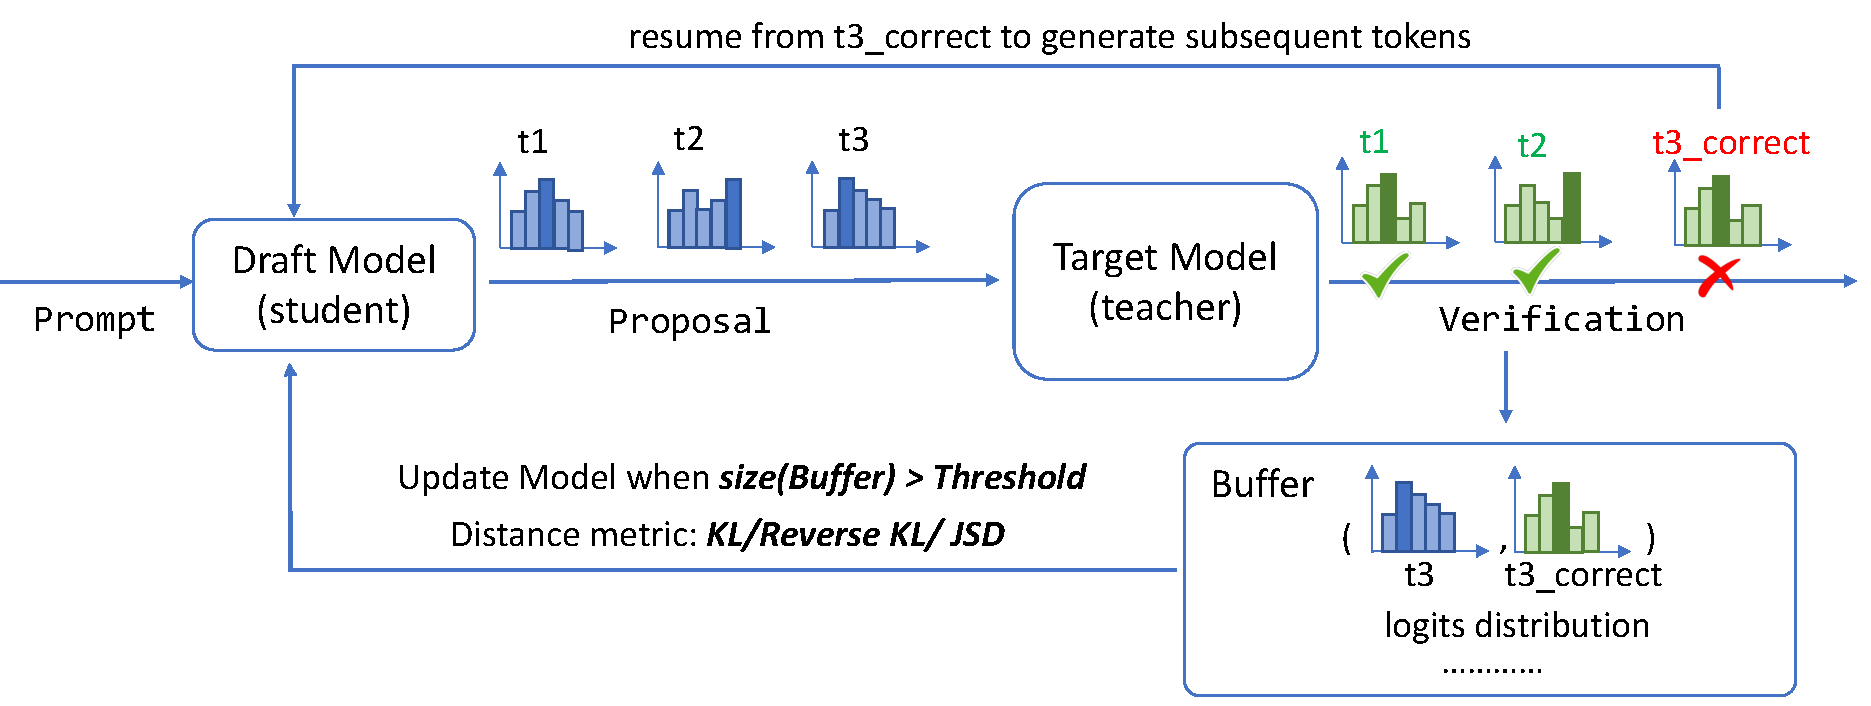
\includegraphics[width=0.8\linewidth]{figures/arch.pdf}
    \caption{Online speculative decoding overview. For each prompt, the draft model suggests multiple tokens in a single step. The target model then verifies these tokens, accepting some and rejecting others. If the student proposes incorrect tokens, both the draft and target distributions are stored in a buffer. Once the buffer exceeds a specified threshold, the draft model is updated by calculating the loss between the draft and target distributions using various distance metrics.}
\end{figure}

In summary, this paper makes the following contributions:
\begin{itemize}[leftmargin=*]
    \item We introduce online speculative decoding to reduce LLM serving latency by adapting (multiple) draft models on the fly using query data and knowledge distillation.
    \item We explore various GKD methods for constructing draft models and identify the most effective variants, suggesting them as superior alternatives to existing finetuning methods in offline settings.
    \item Our method demonstrates a significant improvement in token acceptance rate by 10-65\% on diverse datasets, translating to 1.2-3.1$\times$ reduction in latency theoretically, with a negligible additional cost. It surpasses existing methods which construct static draft models using fine-tuning or distillation on offline datasets, and matches the hypothetical accuracy achieved if all query data were available a priori.
\end{itemize}







\section{Related Work}
LLMs have become pervasive in today's AI applications, underscoring the importance of optimizing LLM inference. 
Numerous system optimizations have been developed to optimize the throughput of LLM serving~\citep{yu2022orca,kwon2023efficient}. This paper particularly concentrates on a significant strand of research, speculative decoding, aimed at reducing the latency of LLM inference.

\noindent \textbf{Speculative decoding.}
Speculative decoding~\citep{leviathan2023fast,chen2023accelerating} accelerates LLM decoding by employing a (small) draft model to predict the outputs of the larger target model, which are then verified by the target model. Typically, the draft model, while having fewer parameters, is pretrained using the same training data as the target mode, resulting in a negotiable inference cost but with compromised capability. 
If the draft model can correctly predict more than one token per verification step, the memory I/O for accessing the model weights and KV cache at inference is amortized across multiple output tokens, thereby reduces latency, especially since LLM inference is often constrained by GPU HBM bandwidth.
The efficacy of speculative decoding largely hinges on the draft model's ability to accurately predict the target model's outputs. Existing work improves the speculation accuracy by using multiple collectively boosted~\citep{miao2023specinfer} or staged~\citep{spector2023accelerating} draft models, or retraining the target model with auxiliary prediction heads as a draft model~\citep{medusa, stern2018blockwise}. These methods predominantly assume a static draft model post-deployment. In contrast, our work introduces a framework that actively adapts the draft model to the evolving user query distribution on the fly, irrespective of the draft model's construction.

\noindent \textbf{Distillation for auto-regressive models.}
Knowledge distillation (KD) is a framework to generate smaller models that emulate the performance of larger models. However, KD in its conventional form has been observed to be less effective for LLMs. \cite{gu2023knowledge} extend KD to autoregressive LLMs by decoding from the student model and optimizing the reserve KL divergence between students and teachers.
Further, \cite{agarwal2023gkd} introduce generalized knowledge distillation (GKD) to optimize a linear combination of the forward KL and reverse KL between teacher and student, using a blend of teacher- and student-sampled data. 
Drawing inspiration from both works, our paper applies KD to speculative decoding for LLMs. We empirically determine the most effective KD variant for maximizing the draft model's accuracy, and extend it to dynamically generate draft models for online LLM services.


\section{Background}

% \subsection{Speculative Decoding}
We first briefly review speculative decoding~\citep{leviathan2023fast}, a critical technique that accelerates inference of a large target LLM $p(\cdot|\vx)$ with token proposals from a small draft model $q_\vtheta(\cdot|\vx)$. 
$\vx$ denotes the concatenation of the input prompt and already generated tokens. %, and $\vy$ denotes the tokens to be generated. 
The two distributions are both auto-regressive. 
We emphasize the parameters $\vtheta$ of the draft model because we usually need to tailor them according to the target LLM for more substantial acceleration. 

% \textbf{Speculative sampling.} 
Speculative decoding uses a (small) draft model to propose $k$ tokens ${\vy} \triangleq \{ y_i\}_{i=1}^k \sim q_\vtheta(\cdot | \vx)$, and let the target LLM estimate the $k+1$ probabilities, $\{p({y}|\vx, {\vy}_{<i})\}_{i=1}^{k+1}$\footnote{${\vy}_{<i}$ refers to $\{ y_j\}_{j=1}^{i-1}$.}, in parallel. %via a forward propagation using casual attention mask \lily{why mention casual attention mask here?}. 
With $i$ rising from $1$ to $k$, speculative decoding accepts the proposal ${y}_i$ if $u \leq  p(y_i|\vx, {\vy}_{<i}) / q_\vtheta({y}_i|\vx, {\vy}_{<i})$ where $u \sim U[0,1]$; otherwise exits. 
Let $a$ denote the number of accepted tokens, which takes values in $\{0,\dots, k\}$. %--- $a=k$ implies all proposals from the draft LLM are accepted by the target LLM. 
We can sample an additional token ${y}_{a+1}$ from the following distribution 
\begin{equation}
p'(y) =
    \begin{cases}
      p(y|\vx, {\vy}_{<a+1}) & \text{if $a = k$}\\
      \mathrm{norm}(\max(0, p(y|\vx, {\vy}_{<a+1}) - q_\vtheta(y|\vx, {\vy}_{<a+1}))) & \text{otherwise}
    \end{cases}       
\end{equation}
where $\mathrm{norm}(\cdot)$ makes the probabilities over the vocabulary sum to $1$. 

Prior work has shown that the resulting samples $\tilde{\vy} \triangleq \{{y}_1, \dots, y_{a+1}\}$ strictly follow the distribution of the target LLM $p(\cdot|\vx)$~\citep{leviathan2023fast}. 
We concatenate $\tilde{\vy}$ to $\vx$ and repeat the above process until meeting ⟨EOS⟩. 
Each run of the target LLM generates $a+1$ tokens with $a\geq0$. This ensures that at least one new token is generated even in the worst case. 
The generation process can be significantly accelerated if the draft LLM better approximates the target one, particularly $a$ is larger for each target LLM run.


\textbf{Expected acceptance rate \& speedup.} 
The acceptance rate, denoted as \(\alpha\), serves as a measure of how closely the draft model approximates the target model. It is defined as the expected probability that speculative decoding will accept a proposal token given the prompt \(y_i \sim q_\vtheta(y_i|\vx, {\vy}_{<i})\). This rate directly influences the expected length ($\E(|\tilde{\vy}|)$) of \(\tilde{\vy}\) for each target LLM run and the speedup brought by speculative decoding. 

Assuming that the \(k + 1\) simultaneous evaluations of the target LLM \(p\) take roughly the same amount of time as generating a single token in parallel, %\woosuk{This assumption may not hold when multiple sequences are batched}
let \(c\) be the time ratio for a single run between \(q_\vtheta\) and \(p\). The expected generation length of a single target LLM run and the speedup in the total wall time due to speculative decoding is represented as~\citep{leviathan2023fast}:
\begin{equation}
\label{eq:gen_len}
    \E(|\tilde{\vy}|) = \frac{1 - \alpha^{k+1}}{1-\alpha},\quad \E(speedup)=\frac{1-\alpha^{k+1}}{(1-\alpha)(kc+1)}.
\end{equation}
% \ion{What is $c$ in the above equation?}
We depict the speedup for varying values of \(\alpha\) in Figure~\ref{fig:analysis-alphas}, which demonstrates the importance of $\alpha$ in affecting the speedup.

\begin{figure}[h]       
    \centering
    \label{fig:analysis-alphas}
    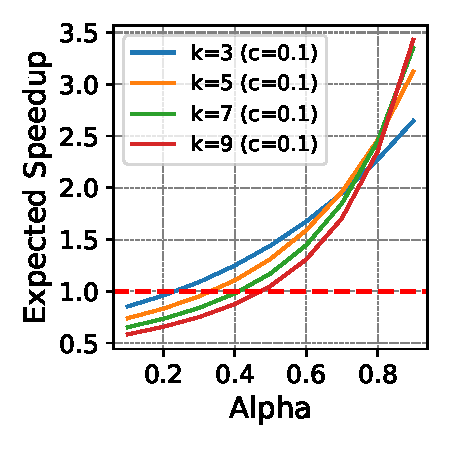
\includegraphics[width=0.25\linewidth]{figures/analysis_k.pdf}
    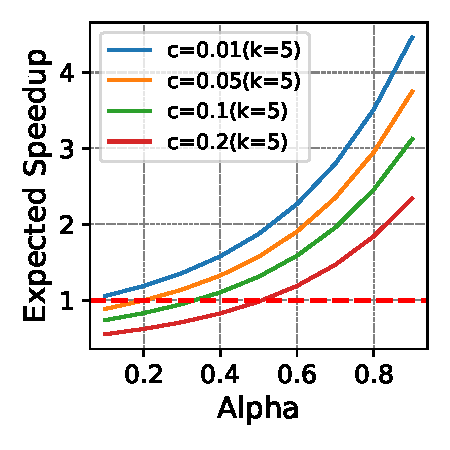
\includegraphics[width=0.25\linewidth]{figures/analysis_c.pdf}
    \caption{Speculative decoding speedups for varying values of \(\alpha\) in Figure~\ref{fig:analysis-alphas}. For smaller \(\alpha\) values, speculative decoding may even degrade performance (indicated by a speedup \(<1\)), particularly when the draft model is sizeable. Furthermore, the relationship between speedup and \(\alpha\) is superlinear; doubling the acceptance rate can yield a speedup exceeding 2$\times$.}
\end{figure}



{\bf Observation.} Interestingly, we can actually enhance \(\alpha\) based on a key observation: the speculative decoding process inherently identifies the inaccuracies of the small draft LLM and offers correct solutions for these inaccuracies. This essentially means that we receive valuable insights on the areas and strategies to refine the draft model at no additional cost. 
Viewed through the lens of online learning, we can effortlessly accumulate a set of input-output pairs, denoted as \( ([\vx, \vy_{<a+1}], p(y|\vx, {\vy}_{<a+1})) \), that have yet to be assimilated by the draft LLM, paving the way for its subsequent optimization. Given the reduced size of the draft model (for instance, it may be over $20\times$ smaller than the target model), its tuning is not only efficient but also viable for real-time online adjustments. 
Prior work~\citep{leviathan2023fast,miao2023specinfer} has primarily approached speculative decoding in an offline manner, meaning the draft model remains static during online deployment. We next develop online speculative decoding to bridge this gap.


% The speculative decoding process automatically detects the errors of the small draft LLM and provides correct answers for replacement. 
% % Namely, the auxiliary information regarding where and how to improve the small draft model is totally free. 
% From a continual/online learning perspective, we can freely collect a set of input-output pairs $([\vx, \vy_{<a+1}], p(y|\vx, {\vy}_{<a+1}))$ that the draft LLM has not learned yet for further model tuning. 
% % Note that the output is of length $1$. 
% This is critical in making low-capacity draft model $q_\vtheta$ better adapt to the dynamic shifts in user intentions in real-world applications. 
% % remains static and cannot adapt to the dynamic shifts in user intentions. This limitation hampers the accuracy and effectiveness of spec decoding in practical scenarios.
% However, such auxiliary information is overlooked by all existing works~\citep{leviathan2023fast,miao2023specinfer}.  \pb{why did they overlook it? provide some intuition -- they probably weren't stupid :)}
% This work will bridge this gap, without incurring excessive computational costs. 


% (a) auxiliary information during the spec process in deployment is wasted by existing works
% (b) the spec distribution cannot vary w.r.t the variation of user intentions in real-world applications.

% In the deployment of spec decoding, existing works often overlook the valuable auxiliary information generated during the process. This auxiliary information is discarded and goes to waste. We argue that by utilizing this auxiliary information, we can significantly improve the performance of the small model without requiring excessive computational resources. 

% Additionally, existing spec decoding approaches fail to account for the variation in user intentions observed in real-world applications. The spec distribution, which governs the suggestions made by the approximation models, remains static and cannot adapt to the dynamic shifts in user intentions. This limitation hampers the accuracy and effectiveness of spec decoding in practical scenarios.

\section{Online Speculative Decoding}
\label{sec:methodology}
We propose the online speculative decoding approach to update the draft model dynamically for more effective suggestions. 
We frame the learning problem based on the aforementioned auxiliary information as online knowledge distillation, where the teacher and student models correspond to the target and draft LLMs in speculative decoding, respectively. 
We elaborate on the details below. 
% With this, the real-time adaptation of the draft model to the query distribution and user intentions is enabled.

% Online speculative decoding as online knowledge distillation.

\subsection{Knowledge Distillation for Speculative Decoding}
\label{sec:knowledge-distill}
Knowledge distillation is a general framework to align the predictive distribution of a small model (i.e., student model) 
with that of a larger one (i.e., teacher model).
Prior research has utilized knowledge distillation to compress neural networks, resulting in decreased inference costs and memory requirements. 
We posit that knowledge distillation is highly effective for speculative decoding. 
In this approach, the draft model acts as the student and the target model serves as the teacher. 
During speculative decoding, we possess complete information on both the proposed and verified probabilities of each token. 
This information helps to construct objectives for distilling the draft model, aligning its output distributions with those of the target model 
and thereby improving the token acceptance rate of the draft model.
% KD, in its original form, is reported to underperform on autoregressive LLMs. 
% \citep{miniLLM} shows that, on many language model tasks, optimizing the reverse KL divergence between students and teachers leads to better performance. 
% This is mainly because LLM inherently captures complex distributions and reverse KL is mode-seeking. 
The distillation loss generally takes the form of:
% This distillation loss is detailed below:
\begin{equation}
    \label{eq:distill}
    \small
    \begin{aligned}
        \ell(\vtheta) &= \frac{1}{n_B}\sum_{\vx^{(i)} \in \mathcal{B}} \ell(\vx^{(i)}, \vtheta), \quad \ell(\vx, \vtheta) =  D ({p(\cdot|\vx)} \Vert {q_\vtheta(\cdot|\vx)} ),% \\
        % &= \frac{1}{n_B}\sum_{\vx \in \mathcal{B}} \sum_{t=1} \KL(q_\vtheta(y_t|\vx, \vy_{<t}) \Vert p(y_t|\vx, \vy_{<t})) \\
    \end{aligned}
\end{equation}
where $\mathcal{B} = \{\vx^{(i)}\}_{i=1}^{n_B}$ denotes a batch of inputs and $D$ denotes some distance measure. 

\textbf{Distance measure.} 
In the case of auto-regressive models, the prediction distribution is categorical at each token. 
Often, we can augment the predicted logits with a tunable temperature $\tau$ for softmax transformation. 
We then use the popular forward KL and reverse KL (RKL), as well as their mixture (i.e., the JSD divergence) 
to instantiate $D$~\citep{agarwal2023gkd,gu2023knowledge}:
\begin{equation}
    \small
    \begin{aligned}
        &\ell_{KL}(\vx, \vtheta) = \KL( {p(\cdot|\vx)}\Vert {q_\vtheta(\cdot|\vx)}), \\
        &\ell_{RKL}(\vx, \vtheta) = \KL({q_\vtheta(\cdot|\vx)} \Vert {p(\cdot|\vx)}), \\
        &\ell_{{JSD}[\beta]} (\vx, \vtheta) = \beta \KL \left({p(\cdot|\vx)} \big\Vert {p}^\beta_\vtheta(\cdot|\vx)\right)+ (1-\beta) \KL \left({q_\vtheta(\cdot|\vx)} \big\Vert {p}^\beta_\vtheta(\cdot|\vx)\right),
    \end{aligned}
\end{equation}
where ${p}^\beta_\vtheta(\cdot|\vx) \triangleq \beta{p(\cdot|\vx)} + (1-\beta){q_\vtheta(\cdot|\vx)}$. 
These objectives diverge from the conventionally used label-based fine-tuning objectives in speculative decoding, 
as highlighted in~\citep{miao2023specinfer, leviathan2023fast}. As shown in Section~\ref{sec:offline-eval},
objectives based on the KL divergence prove to be more effective. This is because distributions 
convey richer information than mere labels, thereby enhancing their capability to guide the student model~\citep{hinton2015distilling}. 
Additionally, these objectives enhance convergence rates~\citep{he2022knowledge} and bolster calibration. 
The reverse KL is highlighted for its mode-seeking behavior, offering unique advantages~\citep{gu2023knowledge}. 
In our study, and in alignment with previous research~\citep{agarwal2023gkd}, we empirically determine that the optimal 
distance measure can vary depending on the tasks and the relative capacities of the teacher and student models (see \S\ref{sec:offline-eval}).


\textbf{Sampling and gradient estimation.}
% \lily{We might want to simplify this section}
Estimating the above objectives involves the expectation over $q_\vtheta(\cdot|\vx)$ or $p(\cdot|\vx)$, which should be expanded recursively. 
Once the recursion depth exceeds $1$, we can not analytically compute $\KL$ but hinge on Monte Carlo approximation. 
% In particular, we draw samples $\vy$ from $p(\cdot|\vx)$, $q_\vtheta(\cdot|\vx)$ or mixture of them for estimating $\ell_{KL}$, $\ell_{RKL}$, $\ell_{JSD[\beta]}$ respectively. 
% This renders the learning resemble a multi-step decision making
When sampling from $q_\vtheta(\cdot|\vx)$, we should differentiate through the sampling process for unbiased gradient estimation. 
\iffalse
E.g.,
\begin{equation}
    \label{eq:grad}
    \small
    \begin{aligned}
        \nabla_\vtheta \ell_{RKL}(\vx, \vtheta) &=  \E_{q} \nabla_\vtheta \log q_\vtheta + \nabla_\vtheta \E_{q_\vtheta} \log \frac{q}{p}= \E_{q} \left[\log \frac{q}{p}  \nabla_\vtheta \log q_\vtheta\right] \\
        &\approx [\log {p(\vy|\vx)} -\log {q_\vtheta(\vy|\vx)}] \nabla_\vtheta [- \log q_\vtheta({\vy}|\vx)].
    \end{aligned}
\end{equation}
It is an unbiased gradient estimator in the same form as policy gradient~\citep{sutton1999policy}, with $\log {p(\vy|\vx)} - \log{q_\vtheta(\vy|\vx)}$ as the reward for $\vy$. 
\fi
However, this leads to policy gradient-style estimators and should rely on elaborate policies such as reward hacking and single-step regularization to reduce gradient variance and stabilize training~\citep{gu2023knowledge}. 

% to reduce gradient variance and stabilize training, elaborate policies such as reward hacking and single-step regularization are introduced~\citep{gu2023knowledge}. 
In comparison, a more straightforward approach is to omit the differentiation through the sampling process~\citep{agarwal2023gkd}, where the sample $\vy$ is directly plugged into the objective:
\begin{equation}
\label{eq:offline}
    \small
    \ell(\vx, \vtheta) \approx
 \sum_{j =1}^{|\vy|+1} D({p(y|\vx, \vy_{<j})} \Vert {q_\vtheta(y|\vx, \vy_{<j})} ).
\end{equation}
This way, various distance measures can be readily applied.
Besides, the sampling becomes disentangled from the distance measure. i.e., we sample $\vy$ from an arbitrary mixture of ${p}(\cdot|\vx)$ and ${q}_\theta(\cdot|\vx)$ but use KL, RKL or JSD for estimating the distribution mis-alignment. 

Intuitively, the samples from the teacher model are usually coherent, which may raise difficulties in fitting the small student model, while samples from the student model may be less structured or even meaningless. 
A workaround strategy is to trade off between them via mixed sampling~\citep{gu2023knowledge}, i.e., $y_j \sim \beta{p(\cdot|\vx, \vy_{<j})} + (1-\beta) q_\vtheta(\cdot|\vx, \vy_{<j})$. 
% Following \citet{gu2023knowledge,agarwal2023gkd}, we can sample $\vy$ from a mixture of $p(\cdot|\vx)$ or $q_\vtheta(\cdot|\vx)$:
% \begin{equation}
%     \vy \sim \rho p(\cdot|\vx) + (1- \rho) q_\vtheta(\cdot|\vx).
% \end{equation}
% Let $\rho$ denote the ratio of the samples from the $q_\vtheta$, which is carefully tuned in our experiments. 
% \zhijie{Do we use token mixture? If so, give the corresponding principle. }



% If we replace the reverse KL with regular KL, likewise, there is:
% \begin{equation}
%     \label{eq:grad2}
%     \small
%     \begin{aligned}
%         \nabla_\vtheta \ell'(\vtheta) &= \frac{1}{n_B}\sum_{\vx \in \mathcal{B}} \nabla_\vtheta \KL(  {p(\vy|\vx)} \Vert {q_\vtheta(\vy|\vx)}) \\
%         &= \frac{1}{n_B}\sum_{\vx \in \mathcal{B}}\E_{p}[ \nabla_\vtheta   - \log q_\vtheta ]\\
%         &\approx \frac{1}{n_B}\sum_{\vx \in \mathcal{B}} \nabla_\vtheta [  - \log q_\vtheta(\tilde{\vy}_i|\vx)],
%     \end{aligned}
% \end{equation}
% where $\tilde{\vy}_i \sim p(\vy|\vx)$ is also an MC sample.




\subsection{Online Knowledge Distillation}
This section expands the application of knowledge distillation for speculative decoding in online environments. 
The approach enables improving the performance of draft model using results from speculative decoding, 
thus dynamically adapting to the query distribution and improving token acceptance rate. 
We also discuss the trade-off of our approach when integrating LLM serving systems.
% The above section details how the knowledge distillation is performed for LLMs in an offline scenario. 
% Here, we describe its extension to the online scenario.
% %, which corresponds to the serving phase of speculative decoding algorithms.  \pb{consider rewriting to avoid passive voice}
% This enables the draft model to learn directly from the query distribution to improve the token acceptance rate.
% We will also discuss how to integrate our approach with existing LLM serving systems to better leverage ``spare flops'' during the serving phase. 


\subsubsection{Algorithm}
\begin{algorithm}[t] 
\caption{Online Speculative Decoding.} 
\label{algo:1}
\small
\begin{algorithmic}[1]
\STATE {\bfseries Input:} 
Target LLM $p(\cdot|\vx)$, draft LLM $q_\vtheta(\cdot|\vx)$, warmup dataset $\mathcal{D}$, online data stream $\mathcal{S}$, guess number $k$, temporary buffer $\mathcal{R}$, replay buffer $\mathcal{Q}$, update interval for the draft model $I$.
\STATE{Pre-train $q_\vtheta$ to approximate $p$ with data from $\mathcal{D}$ by minimizing $\ell(\vx, \vtheta)$ using \cref{eq:offline};}
\STATE{$i \leftarrow 0$;}
\STATE{$\mathcal{Q} \leftarrow []$;}
\STATE{$cur\_len = |\vx|$ // Total sequence length, including prompt length and tokens generated so far.}
\WHILE{True}
    \STATE{$\mathcal{R} \leftarrow []$ // List of ($error\_index$, target logits at $error\_index$) pairs for a single request.}
    \STATE{$\vx \sim \mathcal{S}$, $i \leftarrow i + 1$;}
    \WHILE{⟨EOS⟩ not in $\vx$}
    \STATE{${\vy} = \{{y}_1,...,{y}_k\} \sim q_\vtheta(\cdot|\vx)$;}
    \STATE{Estimate $\{p({y}|\vx, {\vy}_{<i})\}_{i=1}^{k+1}$ in parallel;}
    \STATE{Determine number of accepted tokens $a$ and sample one more token, yielding $\vy=\{{y}_1, \dots, y_{a+1}\}$;} 
    % \STATE{Push $([\vx, \vy_{<a+1}], p(y|\vx, {\vy}_{<a+1}))$ to $\mathcal{R}'$;}
    \STATE{$cur\_len \leftarrow cur\_len + a + 1$;}
    \STATE{$error\_index \leftarrow cur\_len$;}
    \STATE{Append $(error\_index, p(y|\vx, {\vy}_{<a+1}))$ to $\mathcal{R}$;}
    \STATE{$\vx \leftarrow [\vx, {\vy}_{<a+2}]$;}
    \ENDWHILE
    \STATE{Append $(\vx, \mathcal{R})$ to $\mathcal{Q}$;}
    \IF{$i\;\mathrm{mod}\;I = 0$}
    \STATE{Update $q_\vtheta$ on $\mathcal{Q}$ to minimize $\ell(\vx, \vtheta)$ analytically;}
    \STATE{$\mathcal{Q} \leftarrow []$;}
    \ENDIF
\ENDWHILE
\end{algorithmic}
\end{algorithm}

We depict our online speculative decoding algorithm (\tool) in \cref{algo:1}.
\tool begins by training the draft model using the warmup dataset (Line 2). 
The serving system then continuously handles incoming requests (as described in Lines 6 to 23).
For each request, it uses standard speculative decoding (Lines 10-11) to generate responses until the ⟨EOS⟩ token. 
Concurrently, \tool tracks the token index ($error\_index$) and target logits where the draft model proposes the wrong tokens (Line 15). 
Leveraging tracked information, \tool updates the draft model every $I$ iteration, with $I$ being a dynamically adjustable parameter.
\tool updates the draft model with different loss functions (Line 20) as described in Section~\ref{sec:knowledge-distill}.
The choice of loss function depends on the specific (draft, target) model pairs and the corresponding input data. 

{\bf Discussion.} 
% In line 10 of \cref{algo:1}, \tool records the prefix tokens ($[\vx, \vy_{<a+1}]$), which includes the request prompt and tokens generated so far. Moreover, \tool stores logits from the target model at each error location. 
% In practical scenarios, the draft model may commit multiple errors within a single request. 
% For instance, as depicted in Appendix~\ref{}\lily{TODO}, a single execution might generate between \lily{XX} to \lily{XX} tokens. 
% Assuming an output of 100 tokens, this suggests the draft model could err 20 times within a single request (suppose \lily{XX}). 
% Rather than recording the prefixs $([\vx, \vy_{<a+1}])$ after every error, we consolidate prompts with identical prefixes in \(R'\).
% When updating the model, all  $([\vx, \vy_{<a+1}], p(y|\vx, {\vy}_{<a+1}))$ pairs from the same request 
% prompt a singular record for draft model updates. This significant reduction in $R'$ allows \tool to utilize multiple records when updating the draft model in a single execution.
\tool utilizes a replay buffer, $\mathcal{Q}$, to capture all pertinent information for updating the draft model. 
Various eviction policies can be employed to maintain a compact size for $\mathcal{Q}$. 
For example, one could opt to retain only the most informative pairs or the most recent entries. 
Similarly, users have the option to retain data in $\mathcal{Q}$
even after utilizing it to update the model multiple times.
Determining the optimal eviction/retention strategy is a subject for future exploration. 
In the current study, we refrain from evicting any pairs and release $\mathcal{Q}$ after each model update.
% Furthermore, \lily{???}.
Furthermore, $I$ is a dynamic parameter. Depending on the system load and the rate at which the query
distribution changes, users can adjust $I$ accordingly.
For example, we can perform a gradient update opportunistically only when the service traffic is not on spike (i.e., spare flops are available).
% \ion{How does the user adjust exactly?}
Overall, \tool continuously improves the draft model's approximation (indicated by increased token acceptance rate $\alpha$) 
by learning from the target model during the serving phase. We next demonstrate how the enhanced acceptance rate directly 
contributes to a reduction in request latency.


% \pb{broadly, this section needs more care as it is the meat of the paper and the intuition here isn't super clear}

% In the online stage, here are some key differences:
% \begin{enumerate}
%     \item Following the rationale of speculative decoding, We sample $\vy$ from only $q_\vtheta$, on which the distribution mis-alignment is then minimized.
%     \item The online distillation is performed only on the input that the student model $q_\vtheta$ makes mistakes.  \pb{need convincing that this is okay, that we won't overfit on these mistakes}
%     \item The target from the teacher model $p$ of knowledge distillation is free to access.  \pb{access what?}
%     \item The loss $\ell(\vx, \vtheta)$ in the online case can be estimated analytically as the output has only one token. 
% \end{enumerate}


\subsubsection{Latency \& Flops Analysis} 
\label{sec:analysis}
% \alvin{why is this in italics?}
{\bf Latency.} As detailed in  Appendix~\ref{appendix:latency-analysis}, compared with standard speculative decoding, 
the expected speedup for online speculative decoding is  \( \frac{1+\alpha_2+\alpha_2^2+...+\alpha_2^{k}}{1+\alpha_1+\alpha_1^2+...+\alpha_1^k}\).
Based on the data from our experiment (refer to Table~\ref{tab:apha}), when compared to standard speculative decoding, 
we expect a speedup %\ion{Hmm, from the abstract it sounds like the $2.4\times$ speedup is the result of an experiment, but here you are only say it is an estimate} 
improvement for Vicuna-7B (LLaMA-160M as the draft model) by factors of \(2.42\times\), \(1.43\times\), \(1.64\times\), and \(1.22\times\). Similarly, for Flan-T5-XL 3B (T5-small 80M as the draft model), the speedup enhancements are \(3.06\times\), \(1.76\times\), \(2.72\times\), and \(1.55\times\) across the four evaluated datasets. % \woosuk{The sizes of the small models are not provided here.}

{\bf FLOPs.}
% \ion{Isn't this sentence obvious?} \lily{keep for now...}
(1) The FLOPs required to update the draft model are significantly fewer than those needed for inference on a large model. 
As elaborated in Appendix~\ref{appendix:flops}, for the two evaluated model pairs, 
the FLOPs ratio between the target model and the draft model is 18.75 for the pair (LLaMA-160M, Vicuna7B), and 12.6 for the pair (T5-small 80M, Flan-T5-XL 3B). 
%\woosuk{Just curious, how did you select the sizes of the small models? what if you use larger models like LLaMA-1B?}
(2) In practical systems, the FLOPs required for inference are significantly below the machine's capacity.
% \ion{Not sure this example is representative as Arena is woefully inefficient; it needs many GPUs to store many models and not because of the load; in practice, you expect the models to be much better utilized; still, I agree with your point but would be nice to quote also some data from other studies.}
The Appendix~\ref{appendix:flops} provides an analysis of Arena chatbot traces where the cluster's computational utilization is under 1 percent. %\woosuk{I feel this number is a bit exaggerated. The underutilizaiton might be due to the overallocation of GPUs.}
% Consider the Arena dataset (detailed in Appendix~\ref{appendix:arena}). It comprises traces spanning 125 days with 100,000 requests, averaging 2,000 tokens per request (including both prompts and responses).
% When serving a 30B model with 8 A100 GPUs, the FLOPs consumed per second can be estimated as (Still, we estimate 2 FLOPs per token per parameter):
% \[ \frac{2000 \times 100,000}{125 \times 24 \times 3600} \times 30 \times 10^9 \times 2 = 0.55 \times 10^9 \text{ FLOPs or 0.55 GFLOPs} \]
% On the other hand, 8 A100 GPUs offer a combined capacity of \( 8 \times 312 \text{ TFLOPs} \), and the computational utilization is notably low. 
% While Arena may not be the most efficient and might lack substantial traffic, it's the only publicly accessible LLM service trace. 
% Even after amplifying the load multiple times, based on the above calculations, the computation efficiency remains limited.
Given the above two observations, it becomes evident that the FLOPs spent on inference and updating the draft model are relatively 
insignificant when juxtaposed with the FLOPs consumed while operating the target model and the cluster's total FLOPs.


% {\bf Memory.} Assuming we refrain from implementing any eviction/retention strategy for \( \mathcal{Q} \), the maximum size of \( \mathcal{Q} \) is given by \( I \times [|x| + L + \frac{L}{a} \times voscab\_size] \). 




% The data in a temporary buffer $\mathcal{R}'$ should share the prefix, which could be lengthy in some scenarios. 
% Leveraging such a structure, we can perform one single forward propagation for the longest instance in $\mathcal{R}'$ with casual attention mask, and index the output sequence to obtain the logits for the other instances in $\mathcal{R}'$. 
% This way, we can reduce the computational overhead for tuning the draft model for an order of magnitude because, usually, \pb{citation or justification} tens of speculative decoding runs are involved in generating a complete response. 


\section{Experiments}

To assess the efficacy of our method, we initially evaluate its ability to improve the token acceptance rate ($\alpha$) 
within an offline context. 
This provides us with a theoretical upper bound on the performance improvements achievable when the query distribution remains constant. 
Subsequently, we examine the approach's impact in an online environment, discovering that the acceptance rate improves even with a moderate amount of data while maintaining 
accuracy levels comparable to those in the offline scenario. 
Throughout our experiments, we employ two target models ($M_p)$: Vicuna-7B~\citep{vicuna2023} and FLAN-T5-XL (3B)~\citep{chung2022scaling}. Specifically for Vicuna-7B, we utilize LLaMA-160m~\citep{miao2023specinfer} as the draft model ($M_q$). For FLAN-T5-XL, we use T5-Small~\citep{raffel2020exploring} as the draft model. 
We evaluate performance across four diverse datasets: Text-to-SQL (Spider)~\citep{yu2018spider}, graduate school math (Gsm8k)~\citep{cobbe2021gsm8k}, Python code generation (Code-search-Python)~\citep{husain2019codesearchnet}, and financial question answering (Alpaca-finance)~\citep{alpaca-finance}. 
In all experiments, we set the number of proposed tokens to 5 for speculative decoding. For all online experiments, we fix the update interval \( I \) at 8. %

\subsection{Offline Evaluation}
\label{sec:offline-eval}
In this section, we assess the efficacy of employing knowledge distillation to train a small model specifically for speculation in an offline environment. 
In such a setting, the speculative $M_q$ model has unrestricted access to the dataset, and the query distribution remains stable. 
To emulate these offline conditions, we distill the $M_q$ using the training dataset for two epochs and subsequently evaluate its performance by measuring 
the average token acceptance rate ($\alpha$) on the test set.
As detailed in Section~\ref{sec:knowledge-distill}, we evaluated various sampling methods, namely teacher sampling, student sampling, and mix token-level sampling. 
Table~\ref{tab:apha} displays the token acceptance rate of the draft model for each method, using forward KL as the distance metric on the test dataset. 
For comparison, we also provide the acceptance rate for teacher-generated label fine-tuning and the original model.

For both the Vicuna-7B and FLAN-T5-XL models, the teacher sampling method outperforms others by achieving the highest acceptance rate. 
Furthermore, knowledge distillation has proven its efficacy in enhancing the draft model's approximation, resulting in a high token acceptance rate. Intriguingly, we also find that fine-tuning with teacher-generated labels yields impressive performance on the Vicuna-7B model. 
Lastly, we experimented with different distance measurements like reverse KL and JSD. %
Nevertheless, these measurements 
either paralleled or underperformed when compared to forward KL. 
Such empirical findings underscore that the optimal distance measurement or 
sampling method varies depending on the task and model, and we leave to future work to find the best combination. 


\begin{table}
\begin{small}
\caption{Token acceptance rates ($\alpha$) after two epochs. 
{\bf FT}: Finetuning on teacher-generated labels. 
{\bf TF, SF, MixF}: Teacher, student, and mix token sampling respectively, all with forward KL. %
}
\label{tab:apha}
\begin{center}
\begin{tabular}{lllllll}
\toprule
{\bf Model}                 & {\bf Task}         &{\bf Original} & {\bf FT} & {\bf TF }   & {\bf SF }    & {\bf MixF}\\
\midrule
\multirow{4}{*}{Vicuna-7B}  & Spider             &  0.28    & 0.74     & {\bf 0.76}         & 0.62         & 0.70  \\
                            & Gsm8k              &  0.58    & 0.74     & {\bf 0.75}         & 0.67         & 0.73  \\
                            & Code-search-Python &  0.38    & {\bf 0.65}     & {\bf 0.65}         & 0.51         & 0.61  \\
                            & Alpaca-finance     &  0.57    & {\bf 0.68}     & 0.67         & 0.63         & 0.65  \\
\hline
\multirow{4}{*}{FLAN T5-XL} & Spider  &    0.13  &  0.33  & \textbf{0.78}         &      0.67    &  0.70 \\
                            & Gsm8k              &  0.29    &  0.50    & \textbf{0.62}         &   0.51      & 0.55  \\
                            & Code-search-Python &  0.28   &  0.44   & \textbf{0.81}         &    0.67      & 0.78 \\              
                            & Alpaca-finance     &   0.39   &  0.56   & \textbf{0.63}         &    0.59      & 0.60  \\
\bottomrule
\end{tabular}
\end{center}
\end{small}
\vspace{-20pt}
\end{table}


\subsection{Online Evaluation}
\label{sec:eval:online_evaluation}
{\bf Online Learning.} First, we evaluate the effectiveness of our online algorithm by addressing two key questions: (1) Does the online algorithm increase the token acceptance rate? And is this enhancement comparable to the rates achieved in offline settings, which serve as an upper bound given their full access to data? (2) How quickly does the online algorithm increase the token acceptance rate, thereby indicating that the compact model has grasped the underlying distribution?

In our approach, we replicate the online serving process by iterating through the datasets, extracting prompts, and streaming generation requests. The system utilizes speculative decoding for each of these requests. Throughout this serving phase, we continually refine the speculative models, as detailed in Algorithm~\ref{algo:1}.
For our baseline, we envision a scenario where the serving system has the capability to collect data offline in order to distill an initial draft model. This model is subsequently deployed online to cater to future requests. This process is simulated by using 10\% of the dataset to distill the draft model, which remains static during online serving.
For evaluation metrics, we calculate token acceptance rates averaged over the most recent 50 requests. This demonstrates $M_q$'s efficacy on the most current data.

\begin{figure}[h]       
    \centering
    
\includegraphics[width=0.8\linewidth]{figures/legend_figure1.pdf}
    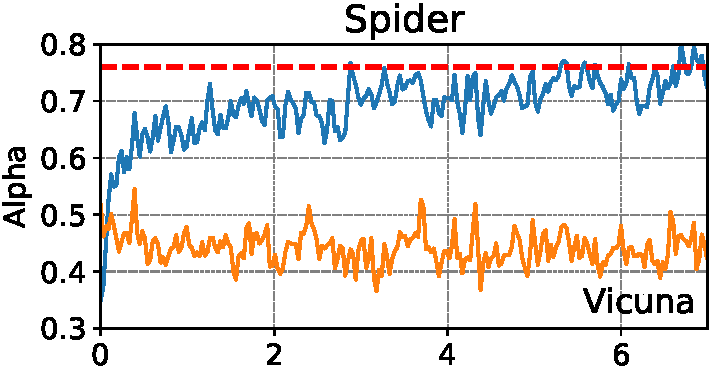
\includegraphics[width=0.256\linewidth]{figures/spider_vicuna.pdf}
    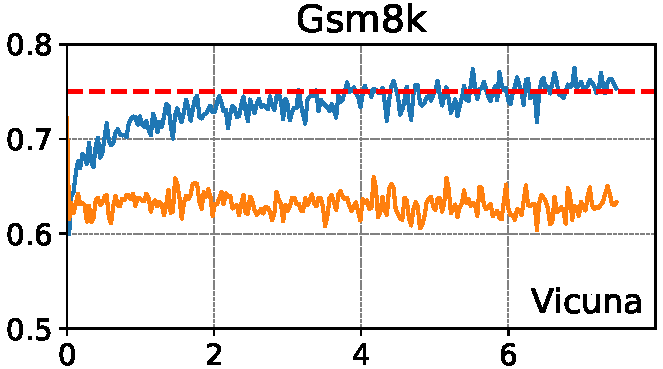
\includegraphics[width=0.242\linewidth]{figures/gsm8k_vicuna.pdf}
    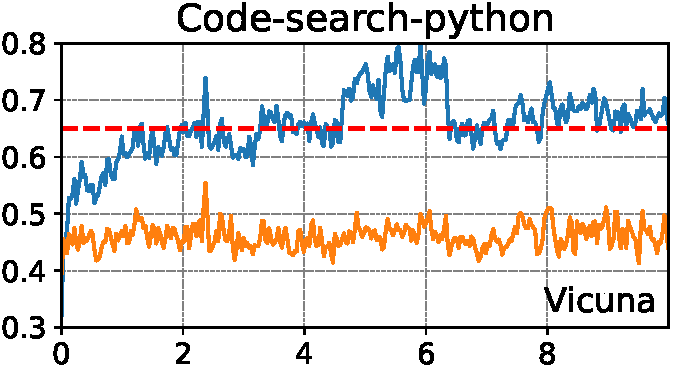
\includegraphics[width=0.24\linewidth]{figures/python_vicuna.pdf}
    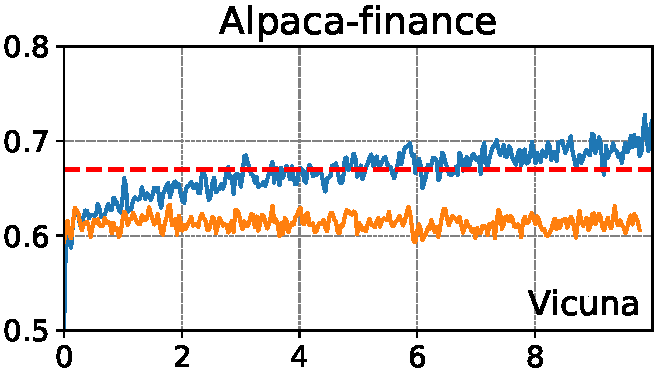
\includegraphics[width=0.24\linewidth]{figures/finance_vicuna.pdf}
    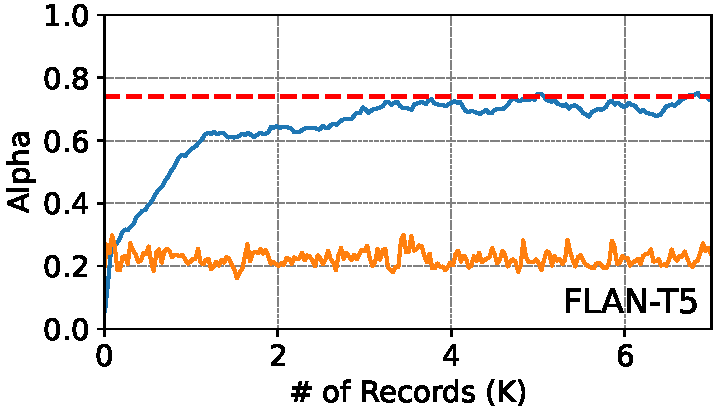
\includegraphics[width=0.259\linewidth]{figures/spider_flant5xl_to_t5small.pdf}
    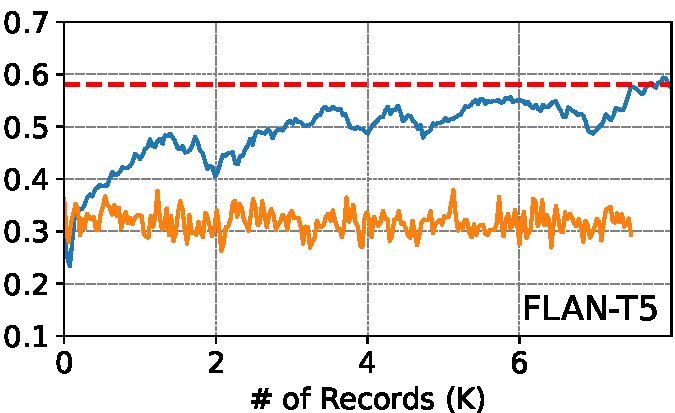
\includegraphics[width=0.24\linewidth]{figures/gsm8k_flant5xl_to_t5small.pdf}
    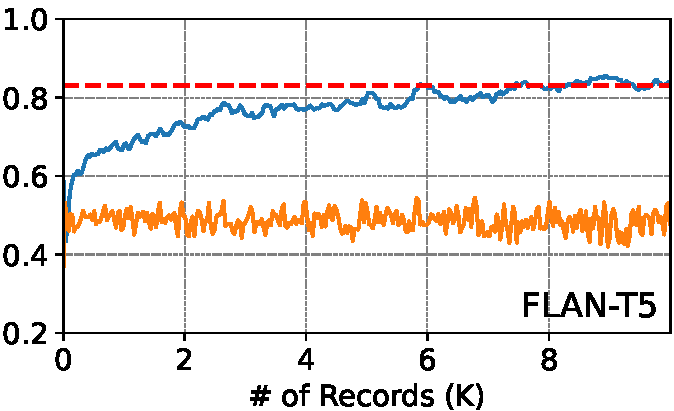
\includegraphics[width=0.24\linewidth]{figures/python_flant5xl_to_t5small.pdf}
    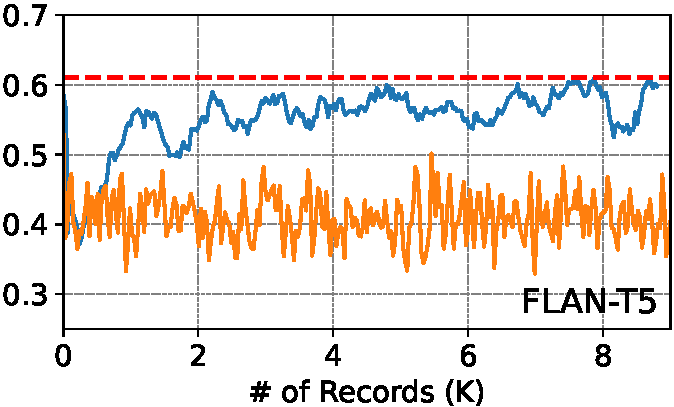
\includegraphics[width=0.24\linewidth]{figures/finance_flant5xl_to_t5small.pdf}
    \vspace{-15pt}
    \caption{Online acceptance rate ($\alpha$) across different datasets. The x-axis represents the number of records that \tool has processed. Alpha is averaged over the most recent 50 records.}
    \label{fig:alphas}
\end{figure}

\begin{figure}      
\vspace{-10pt}
    \centering
    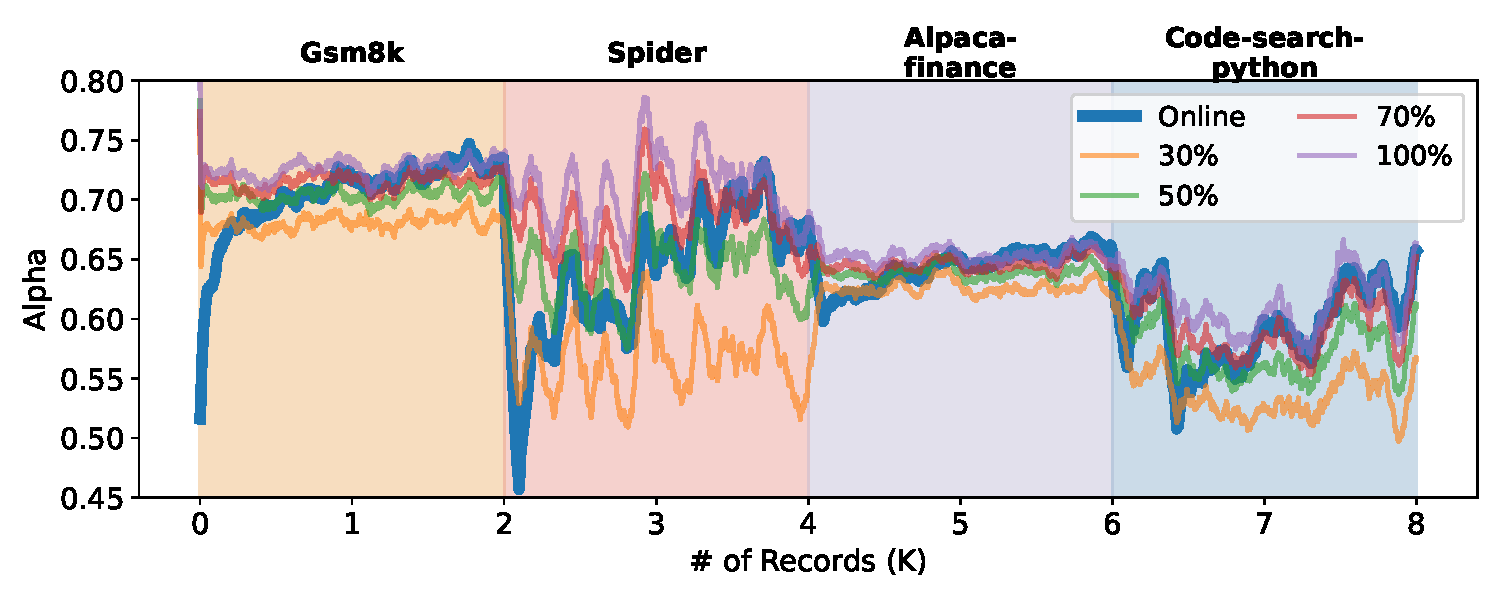
\includegraphics[width=0.75\linewidth]{figures/sharp.pdf}
    \vspace{-15pt}
    \caption{Distribution Shift: Alpha is averaged over the most recent 100 records.}
    \vspace{-15pt}
    \label{fig:dis-shift}
\end{figure}


As depicted in Figure 2, both for Vicuna-7B and FLAN-T5, in the beginning, \tool yields a lower token acceptance rate in comparison to the offline distilled model. Nevertheless, these acceptance rates rise swiftly as the draft model is exposed to more data. We also annotate the token acceptance rate from the offline setting to highlight the potential peak performance that the online serving system could reach. 
In all instances, the online context can achieve comparable results. In some scenarios, \tool even surpasses the token acceptance rate of the offline test alphas. This discrepancy can be attributed to the fact that offline test alphas are assessed on the entire test dataset, whereas the online alphas represent the moving average of the latest 50 requests. It's plausible that \tool performs optimally on specific data subsets, particularly if those subsets are more narrowly distributed than the complete dataset.

{\bf Distribution Shifts.} 
We evaluate \tool's ability to adapt to changes in data distribution. 
We detail the dataset preparation in Appendix~\ref{appendix:distribution-shift}. 
As illustrated in Figure~\ref{fig:dis-shift}, \tool's alpha value dips notably at distribution boundaries, especially around 2K, 4K, and 6K records. 
This is anticipated since the draft model initially struggles when faced with a new distribution. However, the alpha value rebounds quickly as \tool processes more data, highlighting its adaptability to shifting query distributions.

We also compared our results to those from a static setting. To ensure the draft model wasn't just memorizing data, we chose samples distinct from the online evaluation data. These samples correspond to 30\%, 50\%, 70\%, and 100\% of each dataset's online evaluation volume, at 0.6K, 1K, 1.4K, and 2K quantities respectively. As depicted in Figure~\ref{fig:dis-shift}, upon an initial shift in query distribution, \tool's performance aligns with or slightly trails the distillation with 30\% data. However, it quickly catches up, matching or even surpassing performances seen with 70\% to 100\% data access. This highlights \tool's ability to rival models fully exposed to the query distribution, even without intimate knowledge of the underlying query dynamics.


{\bf Real Workloads.} We evaluate \tool on real LMSYS-chat conversations (Appendix ~\ref{appendix:arena}) that span 4 months.
First, we categorize conversations based on the language and we focus on conversations among the top five languages, excluding English. For every chosen language, we use an independent LLaMA-160M to serve as our draft model. All draft models share the same Vicuna-7B as the target model. The token acceptance rate, averaged over the latest 100 requests, showed in Figure~\ref{fig:arena}, reveals that \tool's enhances rates by 0.1 to 0.2, even with under 2K data points. Notably, Japanese was the easiest while Portuguese was the toughest.
We also clustered English conversations by topics using the fine-tuned distilled Bert model~\citep{distill-bert-topic}, focusing on the top five. For topics with over 5K conversations, we sampled evenly to keep it within 5K. Figure~\ref{fig:arena} shows acceptance rates above 0.6 across topics, with Social and Computer discussions peaking near 0.8.
\begin{figure}
    \vspace{-10pt}
    \centering
    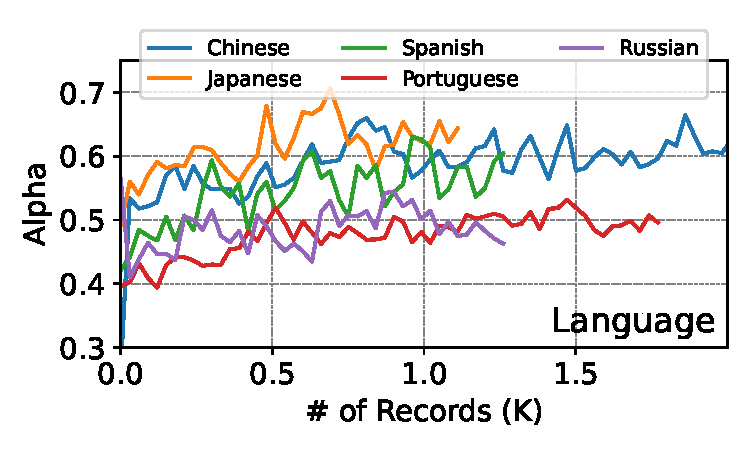
\includegraphics[width=0.4\linewidth]{figures/arena_language.pdf}
    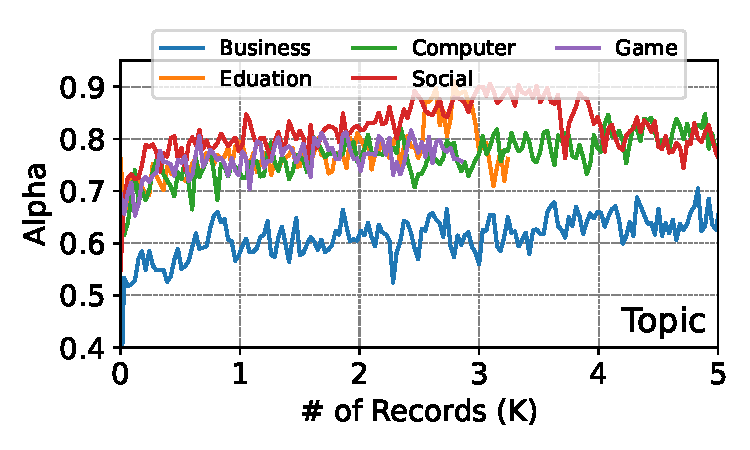
\includegraphics[width=0.4\linewidth]{figures/arena_class.pdf}
    \vspace{-10pt}
    \caption{Chatbot Arena Conversations clustered by language and topic.}
    \label{fig:arena}
\end{figure}

\begin{figure} 
    \vspace{-10pt}
    \centering
    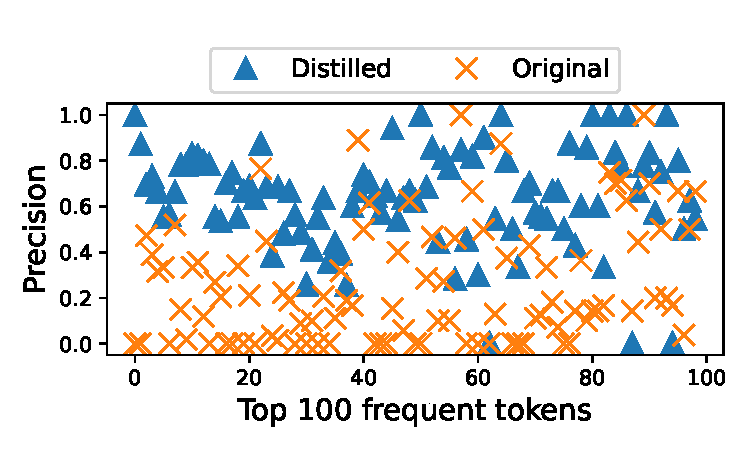
\includegraphics[width=0.4\linewidth]{figures/precision.pdf}
    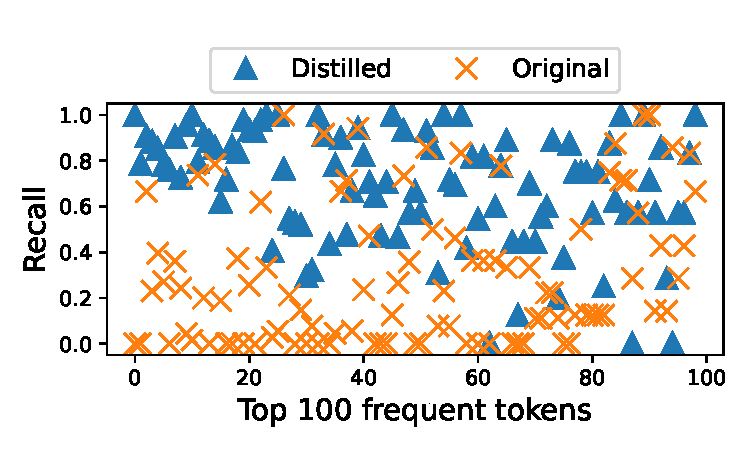
\includegraphics[width=0.4\linewidth]{figures/recall.pdf}
    \vspace{-10pt}
    \caption{Precision and recall of high-frequency tokens. The x-axis shows the rating of the tokens based on their occurrence in the generated answers. For instance, token 1 appears most frequently in answers. Precision = \#  of times token $i$ is accepted by the target model / \# of times token $i$ is proposed by the draft model. Recall = \# of times token $i$ is accepted by the target model / \# of times token $i$ appears in the final answer.}
    \label{fig:freq-acc}
    \vspace{-10pt}
\end{figure}


\subsection{Qualitative Analysis}
In this section, we conduct a comprehensive analysis to understand how our method enhances the token acceptance rate, and which tokens the draft model acquires across varying query distributions.

{\bf High-frequency tokens precision and recall.} In our experiment using the Spider dataset, Vicuna-7M is the target model and LLaMA-160M the draft. 
We identify the top 100 tokens most frequently generated by the target model, which account for 72.2\% of all appearances, 
following a power-law distribution. Figure~\ref{fig:freq-acc} shows a marked improvement in both accuracy and recall
of these tokens after distillation on the test dataset in an offline evaluation. 



\begin{table}[h!]
\vspace{-10pt}
\caption{Top 15 tokens with the most recall/precision improvement across datasets. We ignore \_ before tokens, which represents space in the LLaMA tokenizer.}
\label{tab:tokens}
\begin{center}
\begin{footnotesize}
\begin{tabular}{p{1.5cm}|p{2.4cm}|p{2.4cm}|p{2.4cm}|p{2.4cm}}
\toprule
{\bf Dataset} & {\bf Spider} & {\bf Gsm8k} & {\bf Alpaca-Finance} & {\bf Code-Python} \\
\midrule
{\bf Tokens with the greatest precision increase}
&
AV, SELECT, first, ⟨EOS⟩, template, SUM, G, COUNT, \textbackslash n, city, WHERE, ';, (, IST, id
&
⟨EOS⟩, \textgreater\textgreater, +, To, \textless\textless, this, =, \%, know, are, We, calculate, be, The, have
&
1, Here, (, :, provide, depends, However, goals, amount, 3, there, The, \textbackslash n, personal, will
&
''', (, Here, python, ', how, doc, snippet, import, based, \{, Python, This, :, you \\
\hline
{\bf Tokens with the greatest recall increase}
&
SELECT, *, FROM, (, IST, *), \textbackslash n, COUNT, G, first, WHERE, ⟨EOS⟩, IN, ;, MAX, ';
&
start, \textgreater\textgreater, \textless\textless, +, find, how, we, =, fore, To, so, \textbackslash, ⟨EOS⟩, then, let
&
general, 1, several, This, depends, Here, provide, However, goals, over, (, If, amount, it, can
&
Here, This, snippet, ''', ', how, python, (, takes, Python, you, doc, an, import, def \\
\bottomrule
\end{tabular}
\end{footnotesize}
\end{center}
\vspace{-10pt}
\end{table}

{\bf Tokens learned across different datasets}
In our study, we analyze the top 10 tokens with the most pronounced accuracy and recall improvements across various datasets, focusing on the 100 most frequent tokens to 
understand the draft model's learning trends. As detailed in Table~\ref{tab:tokens}, the improved tokens align well with the underlying data distribution. 
For example, in the Spider dataset, which frequently generates SQL statements, tokens like SELECT and WHERE have notably higher acceptance rates post-distillation. 
Similarly, in the Graduate Math dataset (Gsm8k), tokens such as \textless\textless, \textgreater\textgreater, =, and + stand out. 
These patterns highlight the draft model's ability to adapt and predict tokens consistent with the data distribution.














\section{Conclusion}
Speculative decoding's efficiently hinges on the draft model's approximation to the target model.
We introduce an online speculative method that continuously enhances the draft model based on varying data distributions. Experiments on both synthetic and real data demonstrate that online speculative decoding swiftly adapts to new data distributions, significantly enhancing token acceptance.

\bibliography{iclr2024_conference}
\bibliographystyle{iclr2024_conference}

\appendix
\section{Appendix}
\subsection{Speedup of Speculative Decoding}
As proved in ~\cite{leviathan2023fast}, compared with standard decoding, the expected improvement factor for offline speculative decoding is \(\frac{1-\alpha^{k+1}}{(1-\alpha)(ck+1)}\).
Let the time taken for a single run of \(M_p\) be \(T\). Define \(c\), the cost coefficient, as the ratio of the time taken for a single run of \(M_q\) to that of \(M_p\).
Each execution of lines 7 to 8 takes \(Tck + T\) and, on average, yields \(\frac{1-\alpha^{k+1}}{1-\alpha}\) tokens.
As a result, the average time to produce one token using speculative decoding is given by \(\frac{(ck+1)(1-\alpha)}{1-\alpha^{k+1}}T\). 
In contrast, the time to produce a single token using standard decoding is \(T\). 
Hence, the wallclock time reduction of offline speculative decoding can be described as \(\frac{1-\alpha^{k+1}}{(1-\alpha)(ck+1)}\).

\subsection{Latency Analysis}
\label{appendix:latency-analysis}
Suppose \tool can improve the token acceptance rate from \( \alpha_1 \) to \( \alpha_2 \) %
and $T$ is the generation time for standard decoding. Based on Equation~\ref{eq:gen_len}, this improvement leads to a decrease in the average generation time for each token, transitioning from \( \frac{(ck+1)(1-\alpha_1)}{1-\alpha_{1}^{k+1}}T \) to \( \frac{(ck+1)(1-\alpha_2)}{1-\alpha_{2}^{k+1}}T \). Consequently, this results in a speedup factor of \( \frac{1-\alpha_2^{k+1}}{1-\alpha_1^{k+1}}\frac{1-\alpha_1}{1-\alpha_2} = \frac{1+\alpha_2+\alpha_2^2+...+\alpha_2^{k}}{1+\alpha_1+\alpha_1^2+...+\alpha_1^k}\) compared to standard speculative decoding.

In the aforementioned analysis, we omitted the additional latency due to updating the smaller model for the following reasons:
(1) As illustrated subsequently, the additional computational cost (FLOPs) from the update remains marginal when juxtaposed with the 
computational demands of running the larger model.
(2) Updates are periodic, during times of moderate request loads, the latency for serving individual requests remains largely unaffected. 
Additionally, given that the update operation for the smaller model is considerably less resource-intensive than inference, 
the associated latency might be seamlessly masked, rendering it virtually imperceptible.
Lastly, the processes of updating and inference can even be executed concurrently on separate devices.

\subsection{Flops Analysis}
\label{appendix:flops}
\emph{The FLOPs required to update the draft model are significantly fewer than those needed for inference on a large model.}
Denote \(L\) as the average length of the generated sequence. 
For each verification, the draft model suggests \(k\) tokens. 
The expected length for a single run of the target LLM, denoted as \(a\), can be calculated using Equation~\ref{eq:gen_len}. 
Therefore, \tool undergoes the verification process \(\frac{L}{a}\) times, with each time verifying $k+1$ tokens.
We use \(F_{qfwd}\) to represent the arithmetic operations required by a singular forward run of the draft model for each token, 
and \(F_{pfwd}\) stands for the FLOPs needed for a single forward run of the target model per token.
Therefore, the computational demand (in FLOPs) for the draft and teacher models to handle one request can be expressed as:
$
\text{FLOPs}(draft)  = \frac{L}{a} \times k \times F_{qfwd},
\text{FLOPs}(target) = \frac{L}{a} \times (k+1) \times F_{pfwd}.
$
Let's consider the FLOPs required to update the student model per token as \(F_{qbwd}\). The cumulative FLOPs necessary to process \(I\) requests is given by:
\[
\frac{LI}{a} \times \left[k \times F_{qfwd} + (k+1) \times F_{pfwd}\right] + I \times L \times F_{qbwd}.
\]
Based on the findings of \cite{kaplan2020scaling}, training is approximately three times costlier than inference. This translates to roughly 6 FLOPs per parameter for training on a single token and 2 FLOPs per parameter for inferring on one token. Thus, we can simplify the total FLOPs expression to:
\begin{equation}
    \frac{LI}{a}\left[(k + 3a) \times F_{qfwd} + (k+1) \times F_{pfwd}\right].
\end{equation}

The proportion of FLOPs needed to run the target model to that of the draft model is given by:
\[
\frac{(k+1)\times F_{pfwd}}{(k+3a)\times F_{qfwd}}.
\]
For the two model pairs evaluated, assuming an average of 5 proposed tokens per run: 
(1) (LLaMA-160M, Vicuna7B) with an average acceptance rate of 0.71, the ratio is approximately \( \frac{(5+1) \times 7B}{(5+3 \times 3) \times 160M} = 18.75 \).
(2) (T5-small 80M, Flan-T5-XL 3B), with an average acceptance rate of 0.76, the ratio is roughly \( \frac{(5+1) \times 3B}{(5+3 \times 4.3) \times 80M} = 12.6 \).

\emph{In practical systems, the FLOPs required for inference are significantly below the machine's capacity.} 
Consider the LMSYS-Chat-1M~\cite{zheng2023lmsyschat1m}. It comprises traces spanning 125 days with 1000,000 requests, averaging less than 2,000 tokens per request (including both prompts and responses).
When serving a 30B model with 8 A100 GPUs, the FLOPs consumed per second can be estimated as (Still, we estimate 2 FLOPs per token per parameter):
\[ \frac{2000 \times 1000,000}{125 \times 24 \times 3600} \times 30 \times 10^9 \times 2 = 5.5 \times 10^9 \text{ FLOPs or 5.5 GFLOPs} \]
On the other hand, 8 A100 GPUs offer a combined capacity of \( 8 \times 312 \text{ TFLOPs} \), and the computational utilization is notably low. 
While Arena (the platform that generates LMSYS-Chat-1M) may not be the most efficient and might lack substantial traffic, it's the only publicly accessible LLM service trace. 
Even after amplifying the load multiple times, based on the above calculations, the computation efficiency remains limited.


\subsection{Data Mix}
\label{appendix:data-mix}
Moreover, there is a question of whether the draft model, once adapted to the new distribution, might lose its prior knowledge. 
To probe this, we conducted an experiment mixing 2k prompts each from the Gsm8k and Alpaca-finance datasets. 
During online serving, for the initial 2k requests, we only update the model based on data from the Gsm8k dataset. 
For the subsequent half of the requests, we restrict updates solely to data from the Alpaca-finance dataset. 
We then provide the average token acceptance rates for all requests, segmented by their data source (Gsm8k versus Alpaca-finance).
As depicted in Figure~\ref{fig:mix}, the token acceptance rate for Gsm8k increases as the draft model 
is exposed to more data. Conversely, the acceptance rate (\(\alpha\)) for the Alpaca-finance dataset remains consistent. 
This is anticipated since we only update the draft model using Gsm8k data. In the latter half of the dataset, 
the token acceptance rate for the Alpaca-finance dataset also shows an uptrend. Intriguingly, the rate for Gsm8k remains consistent, 
suggesting that the draft model retains its learned knowledge without showing signs of forgetting.

\begin{figure}      
    \centering
    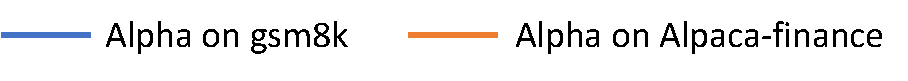
\includegraphics[width=0.48\linewidth]{figures/appendix_legend.pdf} \\
    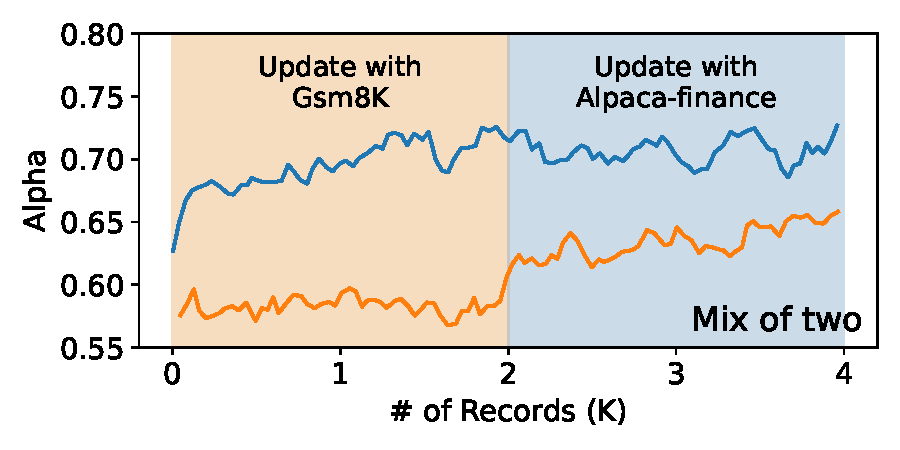
\includegraphics[width=0.48\linewidth]{figures/mix.pdf}
    \caption{Mix of distributions.}
    \label{fig:mix}
\end{figure}

\subsection{Data Preparation for Distribution Shift Analysi}
To emulate this shift in distribution, 
\label{appendix:distribution-shift}
we select 2k prompts from each dataset under evaluation. T
he data from the four datasets are amalgamated by direct concatenation, 
such that the records from $i\times2k$ to $(i+1)\times2k$ belong solely to dataset 
$i$. 

\subsection{Arena Dataset}
\label{appendix:arena}
For expedited experimental evaluation, we randomly sample a subset with 10K records
from LMSYS-Chat-1M~\cite{zheng2023lmsyschat1m}, 
a comprehensive real-world LLM conversation dataset. This dataset encompasses interactions with 25 models spanning 
from April to August 2023 and features conversations in over 150 languages. For all experiments, we only pick conversations for Vicuna models.




\end{document}
